\chapter{Weight and Mass}\label{ch:g4:weight-and-mass}

Astronauts on the \omterm{def:g2:moon-in-the-sky:moon}{Moon} bounced like children on a trampoline,
though they carried heavy packs. Were their packs heavy or \omterm{def:g1:light-and-shadows:source}{light} up
there? To answer properly, we must split an everyday word in two:
what a thing \emph{is made of} --- its \omterm{def:g3:measuring-mass:mass}{mass} --- and how hard the
Earth \emph{pulls on it} --- its \omterm{def:g4:weight-and-mass:weight}{weight}. They are close cousins,
but not twins.

\section{Two ideas hiding in ``heavy''}

You know \omterm{def:g3:measuring-mass:mass}{mass}: how much stuff, in \omterm{def:g3:measuring-mass:units}{grams} and \omterm{def:g3:measuring-mass:units}{kilograms}, judged by
the \omterm{def:g3:levers-and-scales:scale}{balance scale}. And you know the Earth's pull: the no-touch
\omterm{def:g2:pushes-and-pulls:force}{force} that brings every dropped thing down. \omterm{def:g4:weight-and-mass:weight}{Weight} is where the two
meet.

\begin{definition}[Weight]\label{def:g4:weight-and-mass:weight}
The \emph{weight}\index{weight} of a thing is the \omterm{def:g2:pushes-and-pulls:force}{force} with which
the Earth pulls it downward. Weight is what your arm fights when
you hold a bucket, and what stretches the spring when the bucket
hangs from it. Like every \omterm{def:g2:pushes-and-pulls:force}{force}, weight has a direction: straight
down, always.
\end{definition}

\begin{proposition}[More stuff, stronger pull]\label{prop:g4:weight-and-mass:morestuff}
The Earth pulls harder on things that contain more stuff: at the
same place, more \omterm{def:g3:measuring-mass:mass}{mass} always means more \omterm{def:g4:weight-and-mass:weight}{weight} --- two identical
bricks weigh twice what one does. That is why the \omterm{def:g3:levers-and-scales:scale}{balance scale},
which compares the \emph{pulls} on its two pans, manages to compare
\emph{masses}: at one place, equal pulls mean equal stuff.
\end{proposition}

\begin{example}[Cousins, not twins]\label{ex:g4:weight-and-mass:cousins}
\omterm{def:g3:measuring-mass:mass}{Mass} answers: \emph{how much stuff?} It is a property of the thing
alone --- the same in your hand, underwater, or on the \omterm{def:g2:moon-in-the-sky:moon}{Moon}. \omterm{def:g4:weight-and-mass:weight}{Weight}
answers: \emph{how hard is it pulled down here?} It depends on the
thing \emph{and} on where it is. Change nothing but the place, and
the \omterm{def:g3:measuring-mass:mass}{mass} stays; the \omterm{def:g4:weight-and-mass:weight}{weight} can change.
\end{example}

\section{The spring scale}

\begin{definition}[Spring scale]\label{def:g4:weight-and-mass:springscale}
A \emph{spring scale}\index{spring scale} \omterm{def:g2:measuring-length:measure}{measures} \omterm{def:g4:weight-and-mass:weight}{weight} by
letting it stretch a spring: the harder the pull, the longer the
stretch. A pointer beside the stretched spring shows the reading.
Fishermen's scales, luggage scales and the kitchen scale's insides
all work this way --- they feel the \emph{pull}, not the stuff.
\end{definition}

\begin{omfigure}
\begin{tikzpicture}[scale=0.85]
  \draw[thick] (0.6,4.2) -- (2.2,4.2);
  \draw[thick] (1.4,4.2) -- (1.4,3.9);
  \draw[thick] (1.4,3.9) .. controls (1.7,3.75) and (1.1,3.6)
    .. (1.4,3.45) .. controls (1.7,3.3) and (1.1,3.15) .. (1.4,3.0);
  \draw[thick] (1.4,3.0) -- (1.4,2.7);
  \draw[thick, fill=omMeth, fill opacity=0.4]
    (1.0,2.0) rectangle (1.8,2.7);
  \node[right, font=\footnotesize] at (1.95,2.35) {$1$ brick};
  \draw[thick] (5.6,4.2) -- (7.2,4.2);
  \draw[thick] (6.4,4.2) -- (6.4,3.9);
  \draw[thick] (6.4,3.9) .. controls (6.7,3.68) and (6.1,3.47)
    .. (6.4,3.25) .. controls (6.7,3.03) and (6.1,2.82) .. (6.4,2.6)
    .. controls (6.7,2.38) and (6.1,2.17) .. (6.4,1.95);
  \draw[thick] (6.4,1.95) -- (6.4,1.7);
  \draw[thick, fill=omMeth, fill opacity=0.4]
    (6.0,0.3) rectangle (6.8,1.0);
  \draw[thick, fill=omMeth, fill opacity=0.4]
    (6.0,1.0) rectangle (6.8,1.7);
  \node[right, font=\footnotesize] at (6.95,1.0) {$2$ bricks};
  \node[right, font=\small] at (8.0,3.4)
    {double the stuff,};
  \node[right, font=\small] at (8.0,2.9)
    {double the pull,};
  \node[right, font=\small] at (8.0,2.4)
    {double the stretch};
\end{tikzpicture}

{\small A spring feels \omterm{def:g4:weight-and-mass:weight}{weight}: one brick stretches it; two identical
bricks stretch it twice as far.}
\end{omfigure}

\begin{method}[A rubber-band scale]\label{met:g4:weight-and-mass:rubberband}
Build a weight-feeler of your own:
\begin{enumerate}
  \item hang a rubber band from a hook, with a light paper cup
        taped to its bottom;
  \item with the cup empty, mark where the cup's rim stands and
        \omterm{def:g2:measuring-length:measure}{measure} nothing yet: this is the zero mark;
  \item load the cup --- $10$ marbles, say --- and \omterm{def:g2:measuring-length:measure}{measure} with
        your ruler how far the rim sank below the zero mark;
  \item load $20$ marbles and \omterm{def:g2:measuring-length:measure}{measure} again.
\end{enumerate}
Twice the marbles, about twice the stretch: your rubber band
confirms the proposition --- more stuff, stronger pull.
\end{method}

\begin{omfigure}
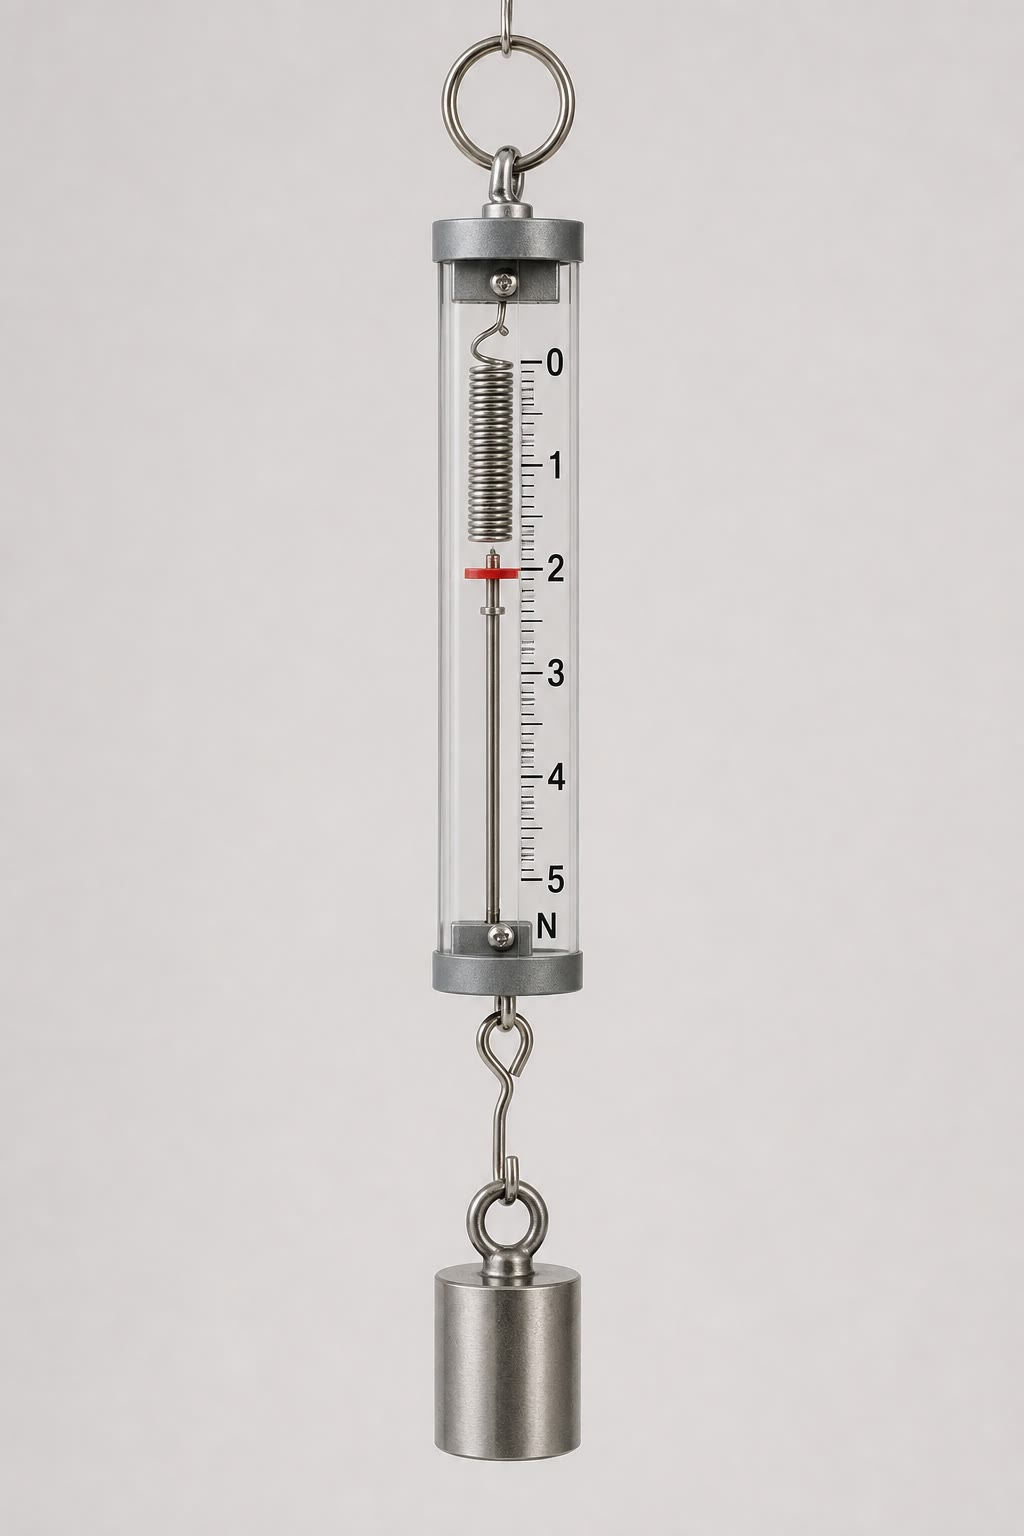
\includegraphics[width=0.3\linewidth]{images/book1/ai/g4-weight-spring-scale.jpg}

{\small A \omterm{def:g4:weight-and-mass:springscale}{spring scale} at work: the load's \omterm{def:g4:weight-and-mass:weight}{weight} stretches the spring, and the pointer turns that stretch into a reading.}
\end{omfigure}

\section{A trip to the Moon}

\begin{example}[The Moon is a weaker puller]\label{ex:g4:weight-and-mass:moon}
The \omterm{def:g2:moon-in-the-sky:moon}{Moon} is much smaller than the Earth, and it pulls things far
more weakly --- about six times more weakly. An astronaut's pack
keeps every \omterm{def:g3:measuring-mass:units}{gram} of its \emph{\omterm{def:g3:measuring-mass:mass}{mass}} on the trip, but its
\emph{\omterm{def:g4:weight-and-mass:weight}{weight}} up there shrinks to a sixth. That is the whole secret
of the bouncing: legs trained to fight Earth-pull suddenly fight a
gentle Moon-pull, and every step becomes a leap.
\end{example}

\begin{omfigure}
\begin{tikzpicture}[scale=0.85]
  \draw[thick] (0.2,0.9) -- (4.2,0.9);
  \draw[thick, fill=omMeth, fill opacity=0.4]
    (1.7,0.9) rectangle (2.7,1.7);
  \node[font=\footnotesize] at (2.2,1.3) {pack};
  \draw[-Stealth, very thick, omDef] (2.2,0.75) -- (2.2,-0.75);
  \node[below, font=\small] at (2.2,-0.95) {on Earth: strong pull};
  \draw[thick] (7.0,0.9) -- (11.0,0.9);
  \draw[thick, fill=omMeth, fill opacity=0.4]
    (8.5,0.9) rectangle (9.5,1.7);
  \node[font=\footnotesize] at (9.0,1.3) {pack};
  \draw[-Stealth, very thick, omDef] (9.0,0.75) -- (9.0,0.5);
  \node[below, font=\small] at (9.0,-0.95)
    {on the Moon: same pack, gentle pull};
\end{tikzpicture}

{\small The same pack --- same \omterm{def:g3:measuring-mass:mass}{mass} --- in two worlds. Only the
pull-arrow changes: \omterm{def:g4:weight-and-mass:weight}{weight} belongs to the place as much as to the
thing.}
\end{omfigure}

\begin{example}[Two scales on the Moon]\label{ex:g4:weight-and-mass:twoscales}
Take both scales to the \omterm{def:g2:moon-in-the-sky:moon}{Moon} and weigh the same pack. The
\emph{spring} scale tells the truth about the place: it reads six
times less --- the pull really is weaker. The \emph{balance} scale
notices nothing: the \omterm{def:g2:moon-in-the-sky:moon}{Moon} pulls the pack and the reference blocks
weakly \emph{alike}, the pans still tie, and it reports the same
\omterm{def:g3:measuring-mass:mass}{mass} as on Earth. Springs feel the place; balances compare the
stuff.
\end{example}

\begin{remark}[Everyday words, physics words]\label{rem:g4:weight-and-mass:words}
In the shop, ``the melon weighs one \omterm{def:g3:measuring-mass:units}{kilogram}'' is harmless talk ---
on Earth, \omterm{def:g3:measuring-mass:mass}{mass} and \omterm{def:g4:weight-and-mass:weight}{weight} travel everywhere together, so nobody is
confused. Physics splits the words because it plans farther than
the shop: for astronauts, for falling things, and --- in a later
year --- for measuring \omterm{def:g2:pushes-and-pulls:force}{forces} in their own proper \omterm{def:g2:measuring-length:measure}{unit}, which will
be named after the scientist who first wrote the law of the Earth's
pull.
\end{remark}

\section{Exercises}

\begin{exercise}[$\star$]\label{exo:g4:weight-and-mass:1}
What question does \omterm{def:g3:measuring-mass:mass}{mass} answer? What question does \omterm{def:g4:weight-and-mass:weight}{weight} answer?
Which one is a \omterm{def:g2:pushes-and-pulls:force}{force}?
\end{exercise}

\begin{exercise}[$\star$]\label{exo:g4:weight-and-mass:2}
Which way does \omterm{def:g4:weight-and-mass:weight}{weight} always pull? What instrument feels \omterm{def:g4:weight-and-mass:weight}{weight} by
stretching?
\end{exercise}

\begin{exercise}[$\star$]\label{exo:g4:weight-and-mass:3}
One brick stretches the \omterm{def:g4:weight-and-mass:springscale}{spring scale}'s spring by two finger-widths.
How far will two identical bricks stretch it? Which proposition
says so?
\end{exercise}

\begin{exercise}[$\star$]\label{exo:g4:weight-and-mass:4}
In the rubber-band scale of
\cref{met:g4:weight-and-mass:rubberband}, why must you mark the
empty cup's position before loading it?
\end{exercise}

\begin{exercise}[$\star$]\label{exo:g4:weight-and-mass:5}
An astronaut carries a pack of \qty{20}{kg} of stuff to the \omterm{def:g2:moon-in-the-sky:moon}{Moon}.
Up there, is its \omterm{def:g3:measuring-mass:mass}{mass} still \qty{20}{kg}? Is it as hard to hold up
as on Earth?
\end{exercise}

\begin{exercise}[$\star$]\label{exo:g4:weight-and-mass:6}
Why could the astronauts leap so high on the \omterm{def:g2:moon-in-the-sky:moon}{Moon}, in spite of
their heavy packs?
\end{exercise}

\begin{exercise}[$\star$]\label{exo:g4:weight-and-mass:7}
On the \omterm{def:g2:moon-in-the-sky:moon}{Moon}, which scale changes its report --- the \omterm{def:g4:weight-and-mass:springscale}{spring scale} or
the \omterm{def:g3:levers-and-scales:scale}{balance scale}? Explain what each one really compares or feels.
\end{exercise}

\begin{exercise}[$\star$]\label{exo:g4:weight-and-mass:8}
True or not: ``A thing with no stuff at all would have no \omterm{def:g4:weight-and-mass:weight}{weight}
anywhere.'' Defend your answer with
\cref{prop:g4:weight-and-mass:morestuff}.
\end{exercise}

\begin{exercise}[$\star$]\label{exo:g4:weight-and-mass:9}
The greengrocer's hanging scale dips as she loads apples into its
pan. Which of the two cousins is her scale feeling? Why does her
trick still sell fair \omterm{def:g3:measuring-mass:units}{kilograms} of apples --- on Earth?
\end{exercise}

\begin{exercise}[$\star\star$]\label{exo:g4:weight-and-mass:10}
A space agency must check that a probe's parts have exactly the
right masses --- but the finished probe will work near a small far
planet whose pull is feeble. An engineer worries: ``Our Earth
weighings will all be wrong out there!'' Reassure him: which
measurements travel unchanged, and which instrument made them?
\end{exercise}

\begin{exercise}[$\star\star$]\label{exo:g4:weight-and-mass:11}
Deep in space, far from Earth, \omterm{def:g2:moon-in-the-sky:moon}{Moon} and Sun alike, an astronaut
lets go of a wrench: it \omterm{def:g1:floating-and-sinking:words}{floats} beside her hand, weightless. Has the
wrench lost its \omterm{def:g3:measuring-mass:mass}{mass}? Give two everyday-style clues she could still
notice showing the stuff is all there. (Hint: try to shake it, or
to throw it.)
\end{exercise}
